To modify the formulation to handle multi-dimensional system or D dimensional trajectories, for instance the 7 joints of an arm or the position of its end effector
we simply use D transformation systems. A key principle in DMPs is to use the same phase system for all the
transformation system, to ensure that the transformation systems are synchronized in time.
Thus the states in the tranformation sytem will be vectors and can be written as:

\begin{subequations}\label{eq:dmpVectSystem}
    \begin{align}
        \tau \vect{\dot{z}}& = \alpha_z (\beta_z \left( \vect{z} - \vect{z_g} \right) - \vect{\dot{z}}) + \vect{f(x)}\label{TVectsystem}\\
        \tau \vect{\dot{y}}& = \vect{z} \\
        \tau \dot{x}& = \alpha_x x\label{cVectSystem}
    \end{align}
\end{subequations}
where the states are vectors of lengths D which are all synchronized in time by the phase equation\eqref{cVectSystem} 

\section{Position Only DMP}
\subsection{2D DMP}
To produce a 2 dimensional DMP in x-y plane, we crated a minimum acceleration trajectory between points
[-3,2] and [3,-2] with initial velocity as [-1,0] which has to be travelled in 5 secs. 
The DMP parameters are: $\alpha_z = 50, N_{bfs} = 100$ with the canonical system parameters as: 
$\alpha_x = 1, \tau = 1$

Minimun acceleration trajectory $x(t)$ is a cubic polynomial in time
\begin{equation}
    x(t) = a_1 t^3 + a_2 t^2 + a_3 t + a_4 
\end{equation}
where $t \leq T $ and the equation is constrained by the boundary conditions $x(0) = x_0, x(T) = x_g , \dot{x(0)} = \dot{x_0} 
\text{ and } \dot{x(T) = \dot{x_g}} $ where $x_0$ and $x_g$ is the initial and final position of the trajectory.


The resultant DMP trajectory is plotted as shown in Fig. \ref{fig:2D_traj}

\begin{figure}[h]
    \centering
    \begin{subfigure}{0.5\textwidth}
        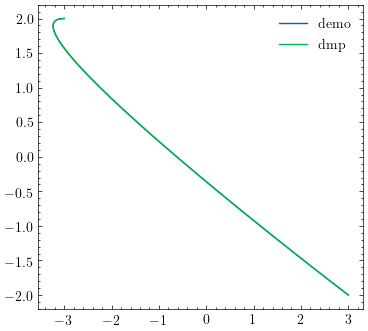
\includegraphics[width=1 \linewidth]{2D_traj.png}
        \caption{2D DMP trajectory}
        \label{fig:2D_traj}
    \end{subfigure}%
    \begin{subfigure}{0.5\textwidth}
        \centering
        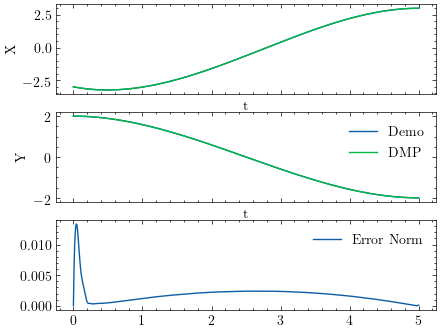
\includegraphics[width=1.2 \linewidth]{2D_traj_error.png}
        \caption{Deviation from the desired trajectory}
        \label{fig:2D_traj_error}
    \end{subfigure}
    \caption{2D DMP trajectory}
    \label{fig:2D_traj}
\end{figure}

\subsection{3D DMP}
Similar to 3D DMP, we can create a 3D DMP in cartesian space by creating a minimum acceleration trajectory for a total time of 5 secs 
between points [-3,-1,1] and [2,3,2] with initial velocity as [0,0,-2].The DMP parameters are: $\alpha_z = 30, N = 100$ with the canonical system parameters as: 
$\alpha_x = 3, \tau = 1$

The resultant DMP trajectory is plotted as shown in Fig. \ref{fig:3D_traj}

\begin{figure}[h]
    \centering
    \begin{subfigure}{0.5\textwidth}
        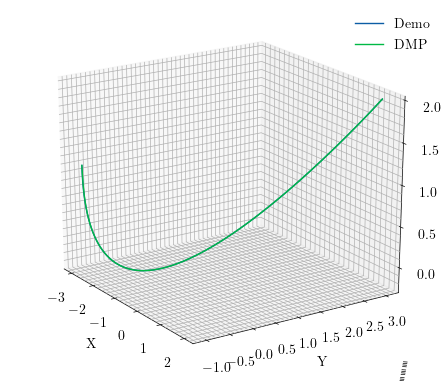
\includegraphics[width=0.9 \linewidth]{3D_traj.png}
        \caption{3D DMP trajectory}
        \label{fig:3D_traj}
    \end{subfigure}%
    \begin{subfigure}{0.5\textwidth}
        \centering
        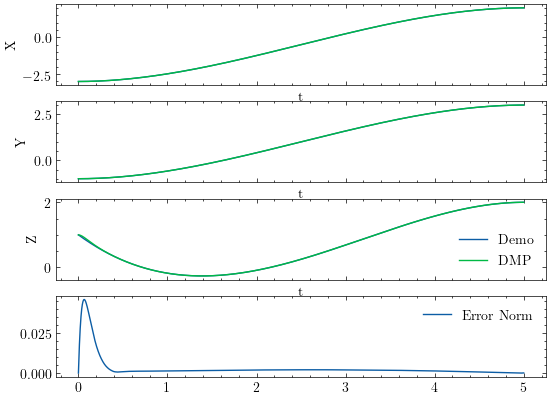
\includegraphics[width=1 \linewidth]{3D_error_traj.png}
        \caption{Deviation from the desired trajectory}
        \label{fig:3D_traj_error}
    \end{subfigure}
    \caption{3D DMP trajectory}
    \label{fig:3D_traj}
\end{figure}

This 3D cartesian DMP can be simulated on a robotic manipulator which follows a certain trajectory.
In this simulation experiment, and all the simulated experiments following, we use Kuka LBR iiwa 
7 axis industrial robot, simulated in PyBullet.
A minimum acceleration trajectory is created between points [0.4,0.4,0.9] and [-0.2,-0.2,1.2] 
 with initial velocity as [0,0.2,-0.1] which has to be travelled in 10 secs. The DMP parameters are:
  $\alpha_z = 20, N = 100$ with the canonical system parameters as: 
  $\alpha_x = 0.5, \tau = 1$

The resultant DMP trajectory simulated is shown in Fig. \ref{fig:3D_only_taj_pybullet}

\begin{figure}[h]
    \centering
    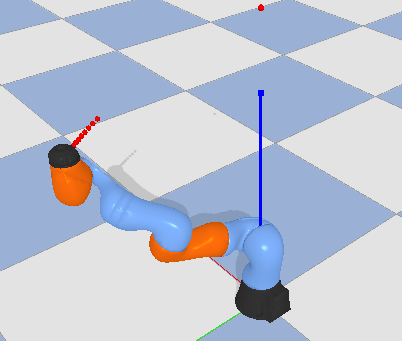
\includegraphics[width= 0.3 \textwidth]{3Dpybullet1.png}\quad
    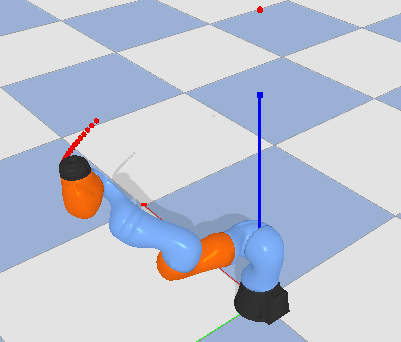
\includegraphics[width= 0.3 \textwidth]{3Dpybullet2.png}\quad
    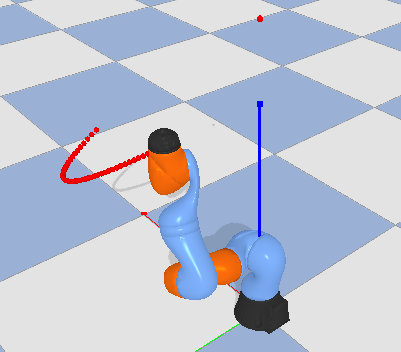
\includegraphics[width= 0.3 \textwidth]{3Dpybullet3.png}

    \medskip

    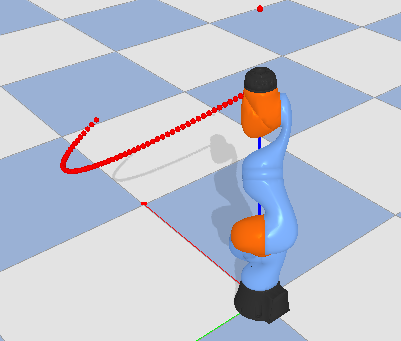
\includegraphics[width= 0.3 \textwidth]{3Dpybullet4.png}\quad
    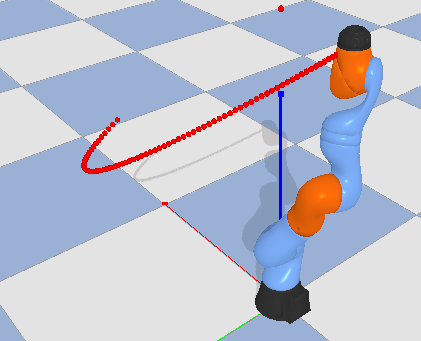
\includegraphics[width= 0.3 \textwidth]{3Dpybullet5.png}

    \caption{3D DMP trajectory simulated on Kuka LBR iiwa 7 axis industrial robot}
    \label{fig:3D_only_taj_pybullet}
\end{figure}

\subsection{Joint Space DMP}
The joint space DMP is a special case where each of the transformation system represents a joint of the robot.
Like previoulsy mentioned the simulation is done on Kuka LBR iiwa. thus the transformation system will be of size 7.
The each joint of the robot follows a sine wave trajectory in time. 

Thus, the desired trajecotry in this case is:
\begin{equation}
    \vect{\Theta(t)} = \vect{\sin(t)} 
\end{equation}
where $\Theta$ is the vector of joint angles and $t \leq T$ where T is the total time of the trajectory.
The parameters of the DMP are: $\alpha_z = 10, N_{bfs} = 1000$ with the canonical system parameters as: 
$\alpha_x = 0.5, \tau = 1$.

The resultant DMP trajectory simulated in DMP is shown in Fig. \ref{fig:joint_traj_pybullet}

\begin{figure}[h]
    \centering
    \begin{subfigure}{0.3\textwidth}
        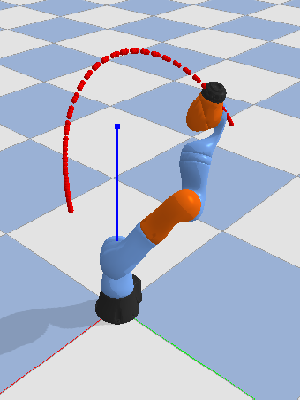
\includegraphics[width=0.9 \linewidth]{jointTraj1.png}
    \end{subfigure}%
    \begin{subfigure}{0.3\textwidth}
        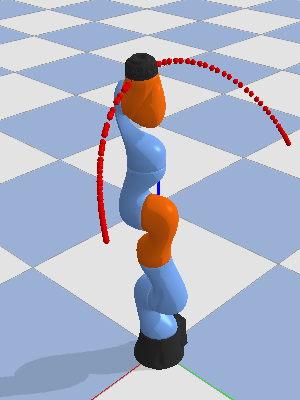
\includegraphics[width=0.9 \linewidth]{jointTraj2.png}
    \end{subfigure}%
    \begin{subfigure}{0.3\textwidth}
        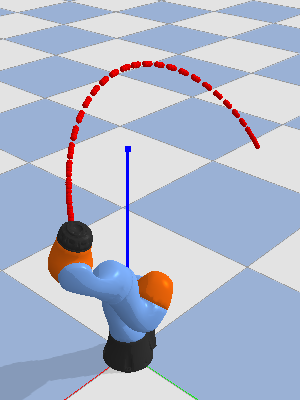
\includegraphics[width=0.9 \linewidth]{jointTraj3.png}
    \end{subfigure}%
    \caption{Joint space DMP trajectory}
    \label{fig:joint_traj_pybullet}

\end{figure}

\section{Orientation DMP}
As mentioned previously, unlike Cartesian positions, the elements of orientation representations are constrained.
And these constraints need to be encoded in the transformation system of DMPs.

There are many ways in which the orientation is represented. In this work, we will use the quaternion representation.

\subsection{Quaternion Representation of DMP}
A quaternion or unit quaternion $\vect{q} = v + \vect{u}$ provides a representation of the orinetation of robots end effector, where The DMP equations for unit quaternion can be represented as:

\begin{align}
    \tau \vect{\dot{\eta}} &= \alpha_z(\beta_z * 2 * log(\vect{g_q} * \bar{\vect{q}}) - \vect{\eta}) + \vect{f_q(x)} \\
    \tau \vect{\dot{q}} &= \frac{1}{2} \vect{\eta} * \vect{q}
\end{align}
where, $\vect{g_q} \in \S^3 $ is the goal orientation, the quaternion conjugate is defined as $\vect{\bar{q}} = v - \vect{u}
\text{and} *$ denotes quaternion multiplication. $\eta$ is the scaled angular velocity $\omega$ and is
treated as unit quaternion with xero scalar component. The logaritminc mapping is defined as:

\begin{equation}
\log{\vect{q}} = 
\begin{dcases}
  \arccos{(v)} \ddfrac{\vect{u}}{||u||} &  \vect{u} \neq 0 \\
  0           &  \text{otherwise} 
\end{dcases}
\end{equation}

The above equations are based on the fact that the unit quaternion that takes $\vect{q_1}$ to $\vect{q_2}$
is given by $\Delta \vect{q} = \vect{q_2} * \vect{\bar{q_1}}$.Unlike with Rotation Matrices the logaritminc mapping defined on $\S^3$ has no discontinuity boundary, just a single singularity
at a sinlg e quaternion $\vect{q} = -1 + [0,0,0]^T $.

The nonlinear forcing term is defined similar to the standard discrete DMP, and is as follows:

\begin{equation}
    \vect{f_q(x)} = \ddfrac{\sum\limits_{i=1}^{N} w_i^o \Psi_i(x)}{\sum\limits_{i=1}^N \Psi_i(x)} = 
    \tau \vect{\dot{\eta}} - \alpha_z \left(  \beta_z * 2 * \log{ \left(  \vect{g_q} * \bar{\vect{q}}\right) } - \vect{\eta} \right)
\end{equation}
where, $w_i^0$ is the weights related to the orientation DMP, and like the discrete DMP can be solved using similar weight calculation methods.

To create a DMP system to reach a desired orientation, we created a orientation trajectory of quaternions using Spherical Liner Interpolation
(SLERP). In SLERP, the quaternions are interpolated using the following formula:

\begin{equation}
    \text{SLERP} = \vect{q_0} \left( \vect{q_0^{-1} q_1} \right)^t
\end{equation}
where $\vect{q_0}$ is the initial quaternion, $\vect{q_1}$ is the goal quaternion, and$\vect{q_0^-1 q_1}$ is 
the quaternion that takes the initial quaternion to the final quaternion. The results of the quaternion DMP where 
$\vect{q_0} =[0.70710678,0,-0.70710678,0] $  is interpolated to 
$\vect{q_g} = [0.37796447 , 0.75592895  ,0.37796447, -0.37796447]$ is shown below.

\begin{figure}[h]
\centering
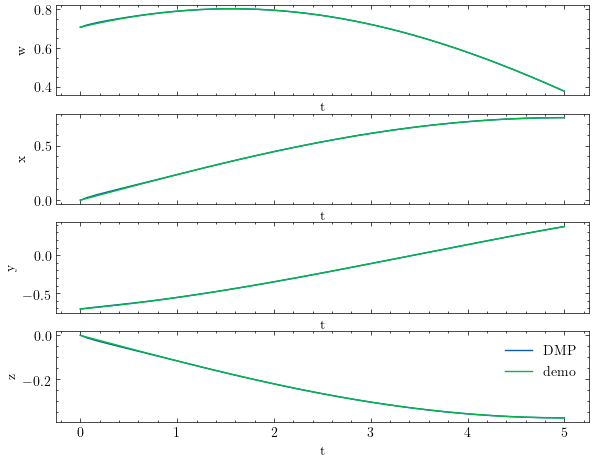
\includegraphics[width=0.7\textwidth]{quaternionDMP.png}
\caption{Quaternion DMP}
\label{fig:quaternionDMP}
\end{figure}




\section{6DOF DMP}
A robot can truly make the most use of its workspace by moving in both cartesian and orientation space. 
Thus it becomes important to implement DMP in 6 DOF. We combined DMPs in Cartesian and Orientation space mentioned in the previous sections to create a 6DOF DMP.
To make the implementation simpler, the demonstrated trajectory, in position and orientation space is recorded and rolled out separately,
then the trajectory followed by the DMP system is then achieved via a cartesian velocity controller. In this section, the robot was moved between initial position [0.4,-0.2,0.8] with 
orientation [-0.17494102, 0.68512454 , -0.17494102 , 0.68512454] 
to final position [-0.2,0.4,1] with orientation [0.2474,-0.1,0.1,0.9689]. The results of this are shown below.

\begin{figure}[h]
    \centering
    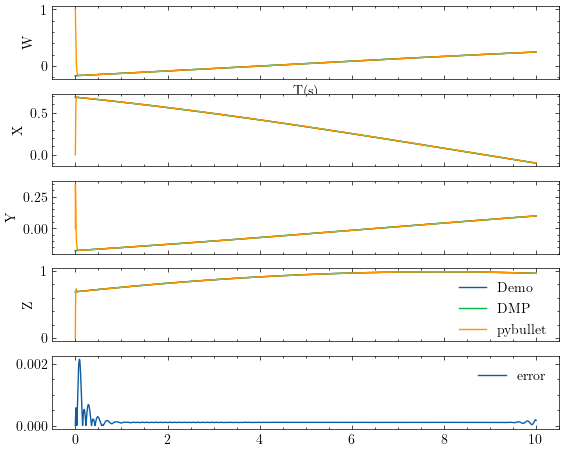
\includegraphics[width= 0.5 \linewidth]{6dof_pos_traj.png}\quad
    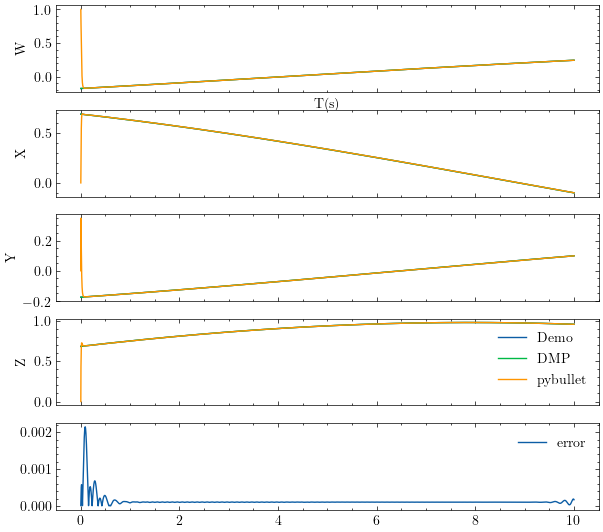
\includegraphics[width= 0.4 \linewidth]{6dof_quat_traj.png}

    \medskip

    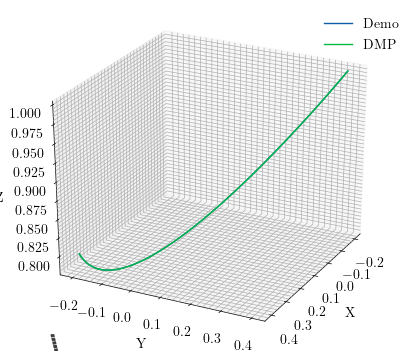
\includegraphics[height= 0.5 \linewidth]{6dof_3D_traj.png}

    \caption{3D DMP trajectory simulated on Kuka LBR iiwa 7 axis industrial robot}
    \label{fig:3D_only_taj_pybullet}
\end{figure}


% \begin{figure}[h]
%     \centering
%     \begin{subfigure}{0.5\textwidth}
%         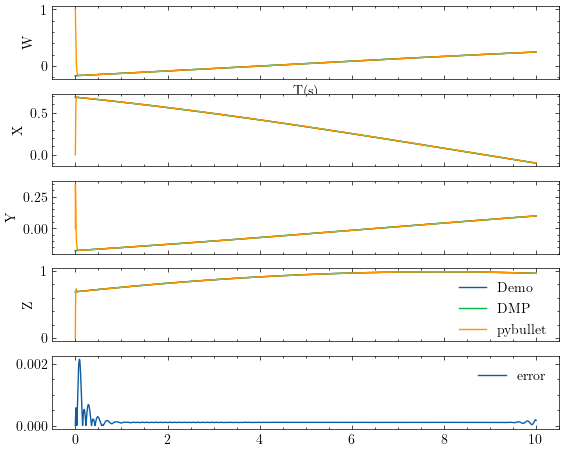
\includegraphics[width=1 \linewidth]{6dof_pos_traj.png}
%         \caption{3D DMP trajectory}
%         \label{fig:6DOF_traj}
%     \end{subfigure}%
%     \begin{subfigure}{0.5\textwidth}
%         \centering
%         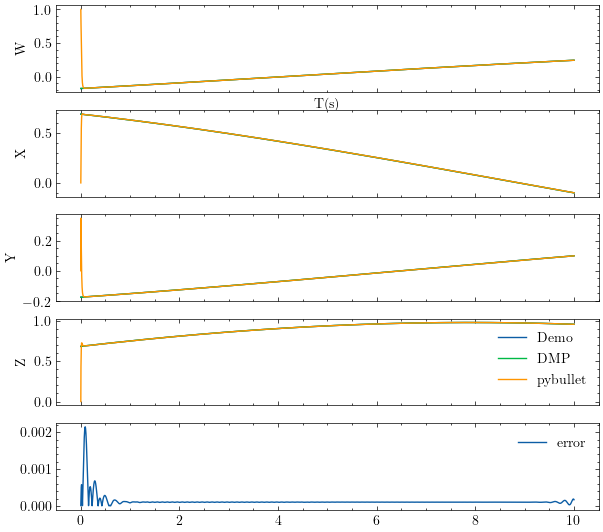
\includegraphics[height=0.8 \linewidth]{6dof_quat_traj.png}
%         \caption{Orientation DMP trajecoctory}
%         \label{fig:6DOF_quat_traj}
%     \end{subfigure}
%     \caption{6DOF DMP trajectory}
%     \label{fig:}
% \end{figure}

% \begin{figure}[h]
%     \centering
%     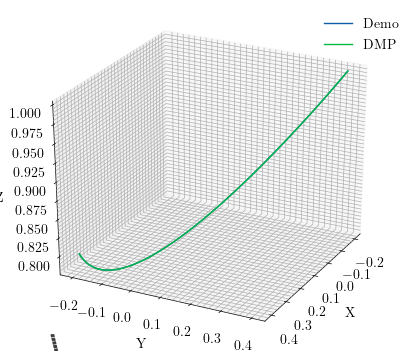
\includegraphics[height=0.5\linewidth]{6dof_3D_traj.png}
%     \caption{3D DMP trajectory for 6DOF DMP}
% \end{figure}

This trajectory was then simulated via Pybullet. A cartesian velocity controller was used in achieving the desired trajectory.
A description of the controller used is given below.

\begin{equation}
    \vect{\dot{q}} = J^{-1} \left( \vect{K_p} (\vect{x_d} - \vect{x}) \right)
\end{equation}
where $J$ is the geometric Jacobian of the system, and $x_d$,$x$ are the desired and current pose of the system. The error 
between the desired and current quaternion in the pose difference is calculated from Eq. \ref{eq:quat_error} , and only the vector term is used
\begin{equation}\label{eq:quat_error}
    \Delta \vect{q} = \vect{q_{des}} * \vect{\bar{q}}
\end{equation}
in the controller. The sign of the real part of the quaternion difference can be multippled to ensure that shortest rotation is followed.
The tuning parameters were, $K_p$ = [55, 55, 55, 44, 44, 44].
The results of the pybullet simulation are shown below.

\begin{figure}[h]
    \centering
    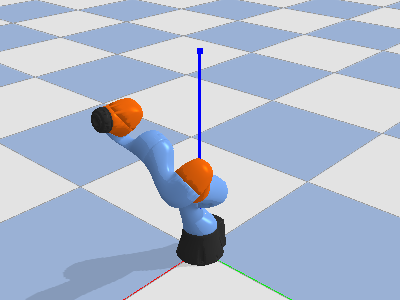
\includegraphics[width= 0.3 \textwidth]{6dof_pybullet1_cropped0.png}\quad
    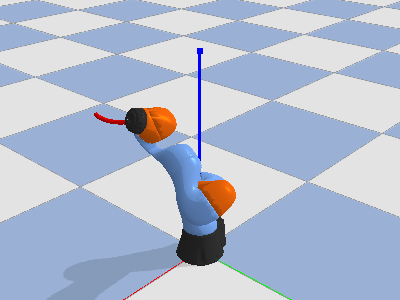
\includegraphics[width= 0.3 \textwidth]{6dof_pybullet2_cropped0.png}\quad
    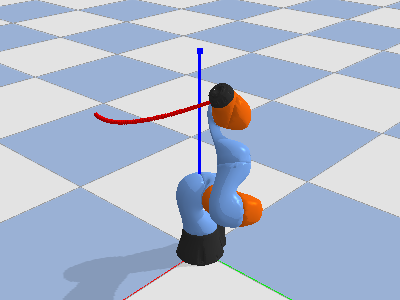
\includegraphics[width= 0.3 \textwidth]{6dof_pybullet3_cropped0.png}

    \medskip

    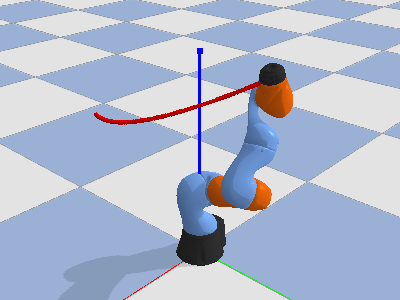
\includegraphics[width= 0.3 \textwidth]{6dof_pybullet4_cropped0.png}\quad
    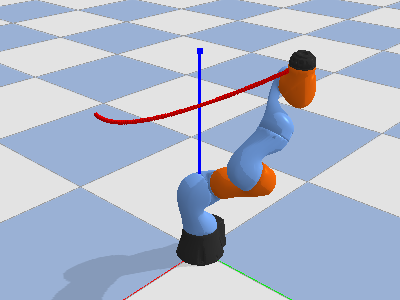
\includegraphics[width= 0.3 \textwidth]{6dof_pybullet5_cropped0.png}

    \caption{6DOF DMP trajectory simulated on Kuka LBR iiwa }
    \label{fig:6DOF_traj_pybullet}
\end{figure}

Next we considered the extension of Dynamic Movement Primitives in the case of Obstacle Avoidance.






















